\externaldocument{eval}

\chapter{Design and Implementation}
\label{chap:implementation}

In this chapter the design and implementation of the prototype for the Austrian parliament are described. First of all, in Section \ref{sec:architecture} the overall architecture and the different components are being discussed. The more detailed description of the implementation is divided into five sections: Section \ref{sec:data_extraction} describes the data extraction from HTML-files, section \ref{sec:transformation} describes the transformation into a structured form, section \ref{sec:export_db} discusses the export to a relational database and the last sections describe the analysis and visualization of the given data.

% Section \ref{sec:data_extraction} which shows how the protocols were accessed, section \ref{sec:transformation} which describes the transformation, section \ref{sec:export_db} which discusses the database export, section \ref{sec:analysis} which describes which analysis is done over the available data and section \ref{sec:visualization} which shows how the information gets displayed.

\section{Architecture}
\label{sec:architecture}
Figure \ref{fig:general_architecture} shows the general architecture of the prototype which was implemented. The Extract-Transform-Load-Application (ETL-Application) brings the data from the debate transcripts in the database whereas the web server application visualizes the results and shows statistics and graphs for the given data. The ETL-Application is implemented using the ETL pattern. This means that there are three distinct steps: Extract - Transform - Load. First the application reads an RSS feed which contains all the protocols for one legislative period and the politician profiles (Extract). The retrieved HTML-files get parsed and are transformed into Java objects (Transform) which get loaded into a relational database\footnote{in the prototype, a PostgreSQL database was used} (Load). To visualize the then available data, the analysis engine queries the database, performs analysis on it and converts the data in a form which can be displayed (e.g. a graph structure). Furthermore, this data is made available via RESTful web services. The Polymer web application \todo{reference section xxxx} accesses these web services and shows graphs and statistics. All the components will be described in more detailed in the following sections.

\begin{figure}
	\centering
	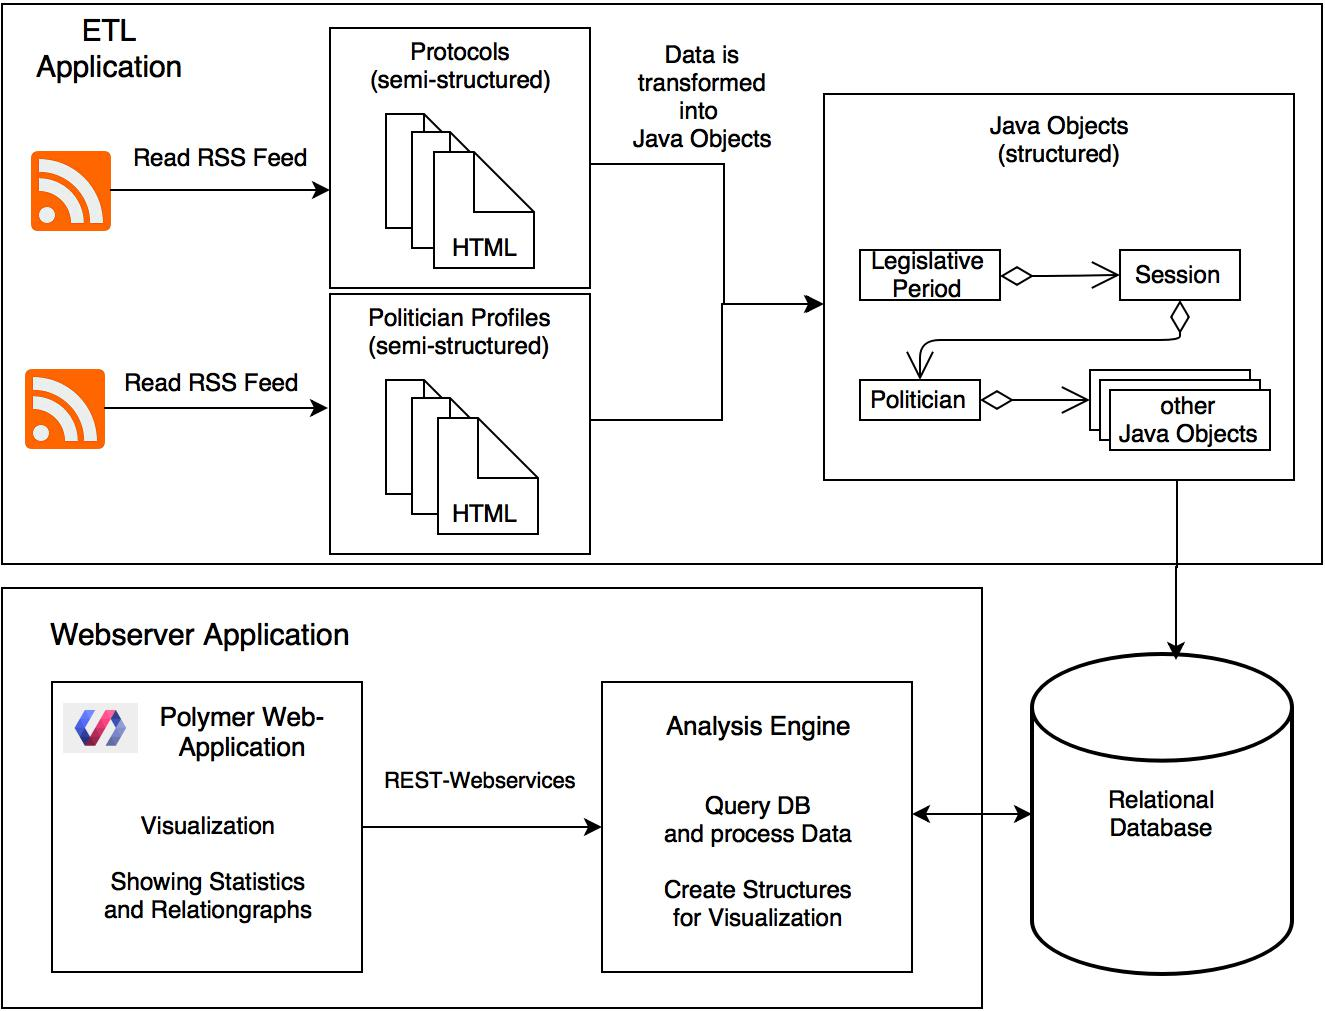
\includegraphics[width=\textwidth]{imgs/overall_architecture}
	\caption{General Architecture}
	\label{fig:general_architecture}
\end{figure}

\section{Data Extraction}
\label{sec:data_extraction}
The first step which has to be done in the ETL-Application is the extraction. The data which is to be transformed has to be collected and stored. In our case the data is contained in the stenographic transcripts of the national council and in politician profiles. Both the protocols and politician profiles are publicly available and can be found at the website of the Austrian parliament (See \url{https://www.parlament.gv.at/PAKT/STPROT/} and \url{https://www.parlament.gv.at/WWER/PARL/}). The protocols are available in PDF-format and since the $20^{th}$ legislative period also in HTML. As the transforming of the PDF-files would not result in sufficient quality, in this thesis only the HTML-files (the data since the $20^{th}$ legislative period) are being extracted and analyzed.

To collect the needed files automatically, RSS feeds are used. There are feeds available for both, stenographic transcripts and politician profiles. The HTML-files which are linked in the feeds are being downloaded and stored on the file system before they are transformed.

\section{Transformation}
\label{sec:transformation}
The next step is the transformation of the HTML-files into Java objects (transformation of semi-/unstructured data to structured data). To be able to extract the desired information out of the HTML-files, the structure of the stenographic protocols and politician profiles was investigated. Then undesired HTML-structures were removed, because they avoided a correct information extraction. For example, the page breaks and page headers in the full text protocols were removed. Finally, the tag structure of the HTML documents and regular expressions were used to find the required data. 
This has proven to be a very challenging task since the transcripts changed over time. For example, in the full text protocols since the $21^{st}$ legislative period, the politicians were referenced with a link to their profile, whereas in the protocols of the $20^{th}$ period, there were only politician names. This made it much harder to find the right politicians as the full list of politicians had to be searched for a politician with the same name and title(s). To transform the HTML-files with good quality, for the protocols of the $20^{th}$ period, there was an extra transformation step which could find the politicians without the link to their profiles.

\subsection{Transformation of the Politician Profiles}
%Figure \ref{fig:politician_profile_example} shows such a Profile. 
For each politician who is sitting in the national or federal council, there exists a politician profile. In the first part of the transformation, all politician profiles are being transformed into a list of politician Java objects. The name (and if provided previous names), the titles, the birth date, and the political mandates are being extracted from the HTML code. Mandates are some kind of political functions like the membership in the national or federal council or the period where the politician was a federal minister. They are of special importance because they include the club memberships of the politician within a specific period of time. 
%To be able to extract these features out of the HTML code, the structure of the HTML file (e.g. the name of the politician is in the first <h1> tag of the page) and regular expressions are used. 
%Figure \ref{fig:politicians_mandates_class_diagram} shows the class diagram of the resulting Java objects, extracted out of the profiles.

%\begin{figure}
%	\centering
%	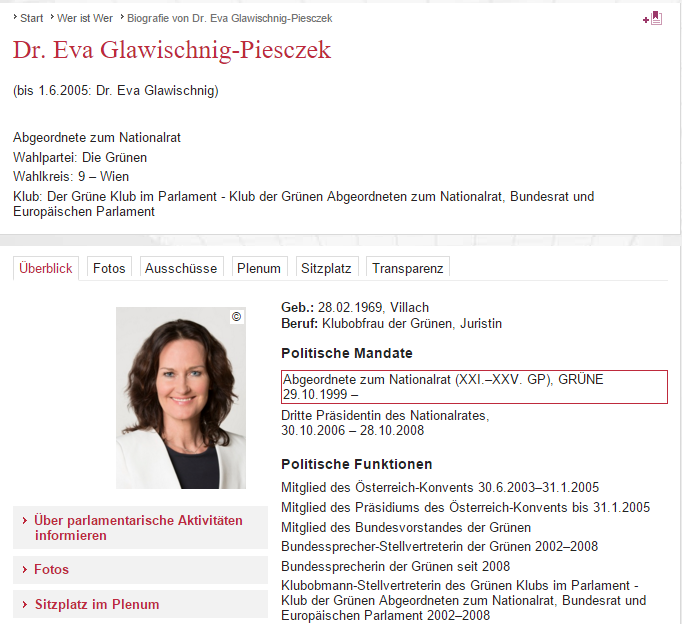
\includegraphics[width=341px]{imgs/politician_profile_example}
%	\caption{Example of a Politician Profile}
%	\label{fig:politician_profile_example}
%\end{figure}

%\begin{figure}
%	\centering
%	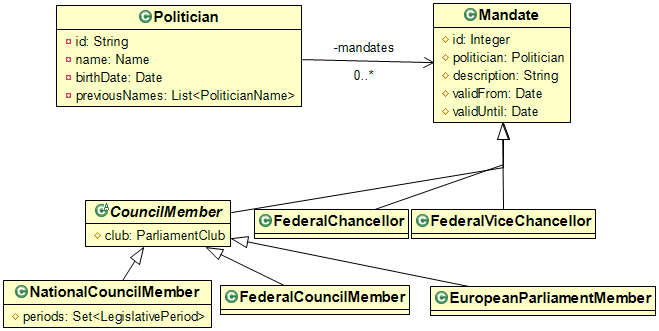
\includegraphics[width=\textwidth]{imgs/politicians_mandates_class_diagram}
%	\caption{Class Diagram of the result of the Profile Transformation Step}
%	\label{fig:politicians_mandates_class_diagram}
%\end{figure}

\subsection{Transformation of the Transcripts}
In the second part of the transformation, the transcripts of the sessions of the national council are transformed. For each session, there exist two files: The full text transcript and the session summary. In the full text transcript every word spoken in a debate is recorded, whereas in the session summary, there is only important information like discussions and speeches summarized. Information that gets extracted out of the protocols includes sessions of legislative periods, chair men in the sessions, politician absences and presences, discussions and speeches of politicians. The list of politicians which was the result of the first transformation part is used to find the politicians in the protocols and to reference them in speeches. %Figure \ref{fig:session_class_diagram} shows the class diagram of the resulting objects of the protocol transformation step.
Figure \ref{fig:all_class_diagram} shows the class diagram of the objects which were extracted in both transformation steps and their relations.

%\begin{figure}
%	\centering
%	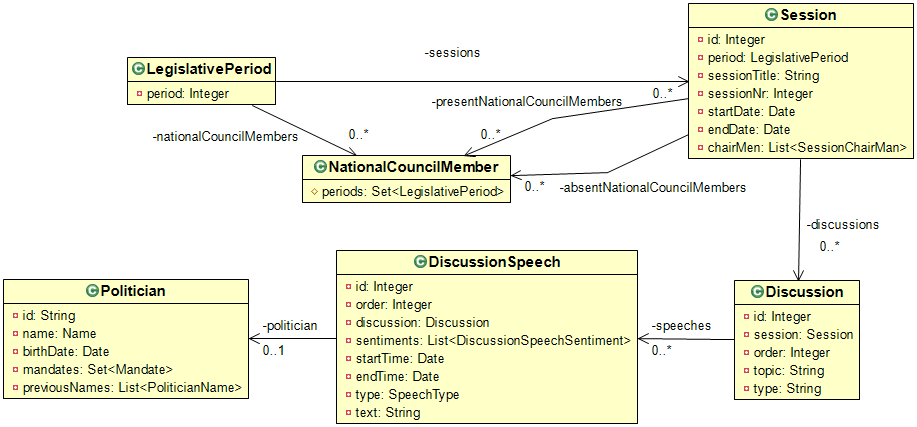
\includegraphics[width=\textwidth]{imgs/session_class_diagram}
%	\caption{Class Diagram of the result of the Protocol Transformation Step}
%	\label{fig:session_class_diagram}
%\end{figure}

\begin{figure}[h]
	\centering
	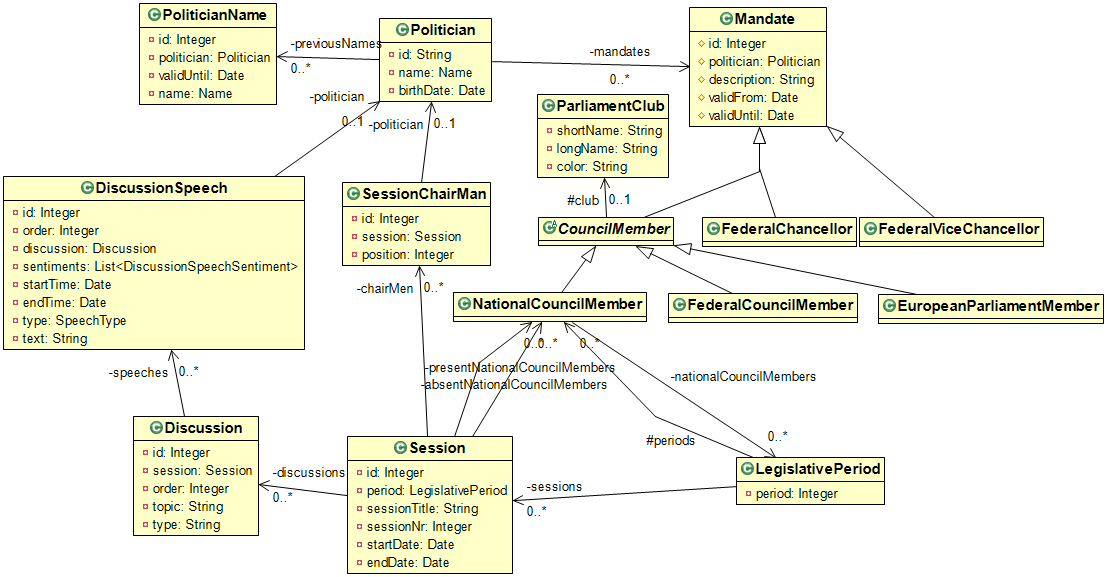
\includegraphics[width=\textwidth]{imgs/all_class_diagram}
	\caption{Class Diagram of the result of the Transformation Step}
	\label{fig:all_class_diagram}
\end{figure}


\section{Export into a Database}
\label{sec:export_db}
The export to a database is the loading part of the ETL-application. The Java objects which were created in the transformation step are being persisted into a relational database. To stay independent of specific databases the Java Persistence API implementation Hibernate\footnote{The Java Persistence API is the standard of OR-mapping in the Java world and Hibernate is an implementation of it.} is used. Using OR-mapping brings the advantages that no SQL-statements have to be written and changes on the tables/objects are easily made using Java annotations.

\section{Analysis}
\label{sec:analysis}
The first step of the analysis phase was to determine which analysis could be applied on the given data. The results can be classified into two categories: simple analysis and network analysis. The simple analysis takes just simple measures like how many speeches a politician held during a legislative period or how often was he absent. These measures are taken via SQL queries on the database built up by the ETL Application. Table \ref{table:simple_analysis} shows all simple analysis measures taken. The network analysis will be discussed in the following sections.

\begin{table}[h]

\bgroup
\def\arraystretch{1.2}
\begin{tabular}{| p{5cm} | p{8cm} |}
\hline
  Name & Description \\
\hline
\hline
  Overall Absence per Period & A percentage of the absence of all national council members in one legislative period. \\
\hline
Absence of a Politician per Period & A percentage of the absence of one national council member in one legislative period. \\
\hline
Absence of a Parliamentary club per Period & A percentage of the absence of all members of one parliamentary club in one legislative period. \\
\hline
Count of Speeches per Politicians and Period & The count of speeches a politician held in the national council during one legislative period. \\
\hline
Mandate Distribution per Period & The assignment of the 183 political mandates to the parliamentary clubs. \\
\hline

\end{tabular}
\egroup

\caption{Simple Analysis Measures}
\label{table:simple_analysis}
\end{table}

\subsection{Politician Relation Graph}
\label{sec:pol_relation_graph}
Network analysis similiar to the one Lucioni \cite{Lucioni_2015} did is done in this thesis. There are measures taken, how strong two politicians are related and the result is shown in a network graph, in which you can visually see the groups of politicians which belong together and how strong the are related, either positively or negatively. Fortunately, all the speeches in the Austrian parliament are tagged with an annotation. A majority of them are tagged with either pro or con, speeches with other annotations are less interesting in the context of this thesis and won't be considered in the following analysis. The pro-con annotations of the speeches are used to create the relation graphs of all the politicians based on their position (pro or con) on the topics of the discussions they held speeches in. The graph shows visually how related two politicians are. If two politicians have a strong positive relationship (if they have the same attitudes in the discussions) they will be displayed close together, but if they have a strong negative relationship (mainly contrary attitudes) they will be displayed far away from each other.

The nodes of this graph are the politicians and the links are the relationships between them, but to create a good network graph, we have to measure the link weight. Lucioni \cite{Lucioni_2015} used the voting data, whereas in the context of the Austrian thesis the speech annotations are used. The strength of a relationship (the link weight $w_p(p_1,p_2)$) between two politicians $p_1$ and $p_2$ is calculated via the following formula:

$$w_p(p_1,p_2) = \frac{\displaystyle\sum_{i=0}^{D} w_p(d_i,p_1,p_2)}{\displaystyle\sum_{i=0}^{D} |w_p(d_i,p_1,p_2)|}$$

where D is the total number of discussions and $d_i$ is the $i^{th}$ discussion. The result $w_p(p_1,p_2)$ is a normalized real number between $-1$ and $+1$, where $+1$ means that the two politicians had the same opinion on every topic and $-1$ means that they have totally contrary opinions. $w_p(d_i,p_1,p_2)$ is the weight of the politicians $p_1$ and $p_2$ in the discussion $d_i$ and can be described by the following formula:

$$w_p(d_i,p_1,p_2) = 
\begin{cases}
    +1       & \quad \text{if } p_1 \text{ and } p_2 \text{ have the same attitude in } d_i\\
    -1  & \quad \text{if } p_1 \text{ and } p_2 \text{ have contrary attitudes in } d_i\\
        0       & \quad \text{if } p_1 \text{ or } p_2 \text{ did not speak in } d_i\\
\end{cases}
$$

In this thesis politician relation graphs get built for all legislative periods, to be able to view the structure of each period separately. To achieve to get a graph for only one period, only the discussions of this period were taken into account. The nodes of such a graphs are the politicians and the links are the relations between the politicians. There exists a link between two politicians if they spoke at least once in the same discussion.

\subsection{Parliamentary Club Relation Graph}
\label{sec:club_relation_graph}
Similar graphs can be constructed for the parliamentary clubs. These graphs show how the clubs are related to each other. The weights of the links of these graphs are computed by summing all weights of the politicians of the clubs $c_1$ and $c_2$ and normalizing the sum. This can be expressed using the following formula:

$$
w_c(c_1,c_2) = \frac{\displaystyle\sum_{i=0}^{D} w_c(d_i,c_1,c_2)}{\displaystyle\sum_{i=0}^{D} |w_c(d_i,c_1,c_2)|}
$$

$$
w_c(d_i,c_1,c_2) = \frac{\displaystyle\sum_{i=0}^{P_{c_1}} \displaystyle\sum_{j=0}^{P_{c_2}} w_p(d_i;p_{c_1,i};p_{c_2,j})}{\displaystyle\sum_{i=0}^{P_{c_1}} \displaystyle\sum_{j=0}^{P_{c_2}} |w_p(d_i;p_{c_1,i};p_{c_2,j})|}
$$

The result $w_c(c_1,c_2)$ is again a normalized number from $-1$ to $+1$ and describes how the clubs are related. $P_{c_x}$ describes the count of the politicians which belong to $c_x$ and $p_{c_x,y}$ is the $y^{th}$ politician which belongs to the parliamentary club $c_x$. Analogously to $w_p(d_i,p_1,p_2)$, $w_c(d_i,c_1,c_2)$ describes the weight of the clubs $c_1$ and $c_2$ in the discussion $d_i$ and is also in the range of $-1$ to $+1$.

\subsection{Pre-Calculation of Relation Weights}
The calculation of all weights for the relations is quite expensive, as there are $\frac{n * (n - 1)}{2}$ weights which have to be calculated for every discussion (n is the number of politicians which spoke in the discussion). So, if a graph should be displayed, it would take too long to compute all these weights then. To handle this problems all politician relation weights $w_p(d_i,p_1,p_2)$ are calculated and persisted into the database immediately after new data is available (after the loading step of the ETL Application). When the data is needed to show the graph the database gets queried and using the aggregation functions of the database $w_p(p_1,p_2)$ and $w_c(c_1,c_2)$ can be easily derived for each pair of politicians and parliamentary clubs in an arbitrary period of time.

\subsection{Other Analysis with the Relation Weights}
With the now available weights between the politicians and parliamentary clubs also analysis other than the relation graphs can be applied. By summing all the weights where one politician is in the government whereas the other one is in the opposition, a general tendency on how distinct government and opposition are can be calculated. See the results in section \ref{sec:gov_opp_relation}. Another measure which can be taken out of the relation weights is the affinity of a politician to a certain party by again summing all the weights of the politician and all the politicians of the party. Furthermore, also the most and least related politicians of a politician can be derived by sorting all the calculated weights $w_p(p_1,p_2)$.



\section{Visualization}
\label{sec:visualization}
The visualization of the extracted data was an important task because only if the data is shown in a proper way it will potentially address a broad spectrum of people. That's why there was a big empathize on the data representation. Another requirement was that the application should run on as many devices as possible. Therefore a web application was implemented, as it will be accessible for almost anybody in the world, as long as he/she has a device with internet and a browser. A few web frameworks were evaluated and it was chosen an architecture with Spring Boot in the back end offering JSON/REST web services and Polymer in the front end for the visual representation.


\subsection{Navigation Concept}
Figure \ref{fig:navigation_concept} shows the navigation concept of the implemented prototype. The start page shows an overview of the available pages and short statistics for the current legislative period like the mandate distribution and the overall absence. From the start page it is possible to navigate to the politician overview, the legislative period overview, the politician and the parliamentary club relation graph pages. 

The politician overview shows the members of the national council of a period, which can be specified. For each politician, the absence percentage and the speech count in this period is presented. If a politician is selected the politician's detail page gets opened. There is general data of the politician, the political mandates and the most/least related politicians shown.

The legislative period overview shows all legislative periods which were considered for this thesis (all from the $20^{th}$) with short statistics. If a period gets selected, the period detail page where also a ranking of the most active and most absent politicians and clubs is shown.

On the politician and club relation graph pages there are graphs for the selected periods. In the politician relation graph there is also the possibility to filter for a specific topic of a discussion. Furthermore, a minimum count of speeches two politicians have spoken in common, before their relation is shown in the graph can be set. This creates the possibility to have a cleaner graph which only shows relations which are known to be correct until a certain degree.

\begin{figure}
	\centering
	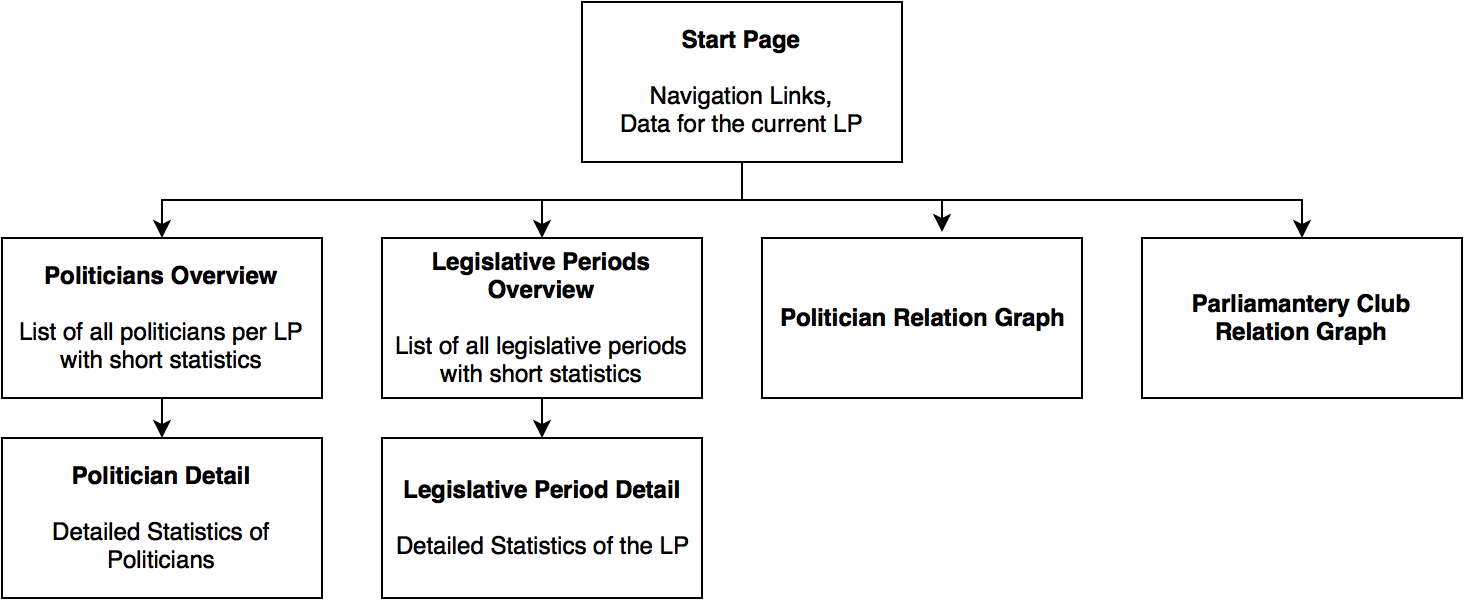
\includegraphics[width=\textwidth]{imgs/navigation_concept}
	\caption{Navigation Concept of the Web Application}
	\label{fig:navigation_concept}
\end{figure}

\subsection{Relation Graphs}
The relation graphs\footnote{See sections \ref{sec:pol_relation_graph} and \ref{sec:club_relation_graph} for the creation of the graphs and chapter \ref{chap:evaluation} for the resulting graphs.} were visualized using force layout design graphs of the d3 JavaScript library. As Bostock \cite{d3_2011} describes in his paper about d3, the force layout is built with an algorithm proposed by Dwyer \cite{Dwyer_2009}, which combines physical simulation and iterative constraint relaxation to show graphs with edges with different desired length. 

The nodes of the graphs are the politicians/clubs and the edges were the relations between them. The more positive the relationship between two nodes is the closer they appear together in the graph. The relationship between two nodes is described with the weights $w_p$ and $w_c$, respectively (see sections \ref{sec:pol_relation_graph} and \ref{sec:club_relation_graph}). So if the weight of the edge is $+1$ the desired length of the edge would be zero, whereas if the weight would be $-1$, the desired length would be a predefined maximum value (the maximum graph dimension is used in the prototype).

The calculated graph data is given into the algorithm of the d3 force layout graph and the algorithm tries to show a graph with the desired length of each edge. It improves the result iterative, this means that the graph looks better and better the more iterations were walked through. The result of the algorithm is then a more or less stable graph, where strong positive related nodes appear close to each other and negative related nodes appear far away from each other. This gives the possibility to identify communities of politicians which have similar attitudes and opinions.

